\documentclass[border=5pt,tikz]{standalone}
\usepackage{amsmath} % for \dfrac
\usepackage{physics}
\usepackage{tikz,pgfplots}
\pgfplotsset{compat=1.18}
%\usepackage[outline]{contour} % glow around text
\usetikzlibrary{arrows,arrows.meta}
\usetikzlibrary{decorations.markings}
\usetikzlibrary{hobby}
\usepgfplotslibrary{fillbetween}
\tikzset{>=latex} % for LaTeX arrow head
\usepackage{xcolor}


\begin{document}

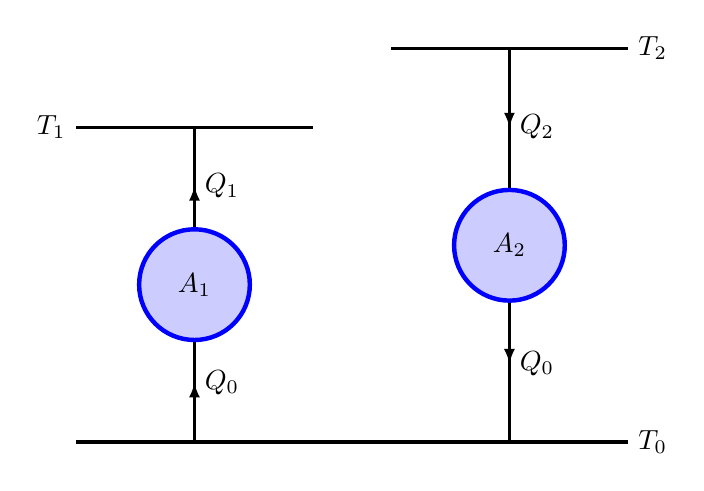
\begin{tikzpicture}
    \begin{scope}[thick, decoration={
    markings,
    mark=at position 0.5 with {\arrow{>}}}
    ] 
        \draw[very thick, black] (0, 0) -- (7, 0) node[right] {$T_0$};
        \draw[very thick, black] (0, 4) node[left] {$T_1$}-- (3, 4) ;
        \draw[very thick, black] (4, 5) -- (7, 5) node[right] {$T_2$};
        
        \draw[postaction={decorate}] (1.5,0)-- node [right] {$Q_0$} (1.5,1.5) ;
        \draw[postaction={decorate}] (1.5,2.5)-- node [right] {$Q_1$} (1.5,4);
        %\draw[postaction={decorate}] (2.5, 2) --node[above] {$W$} (4.7, 2) ;
        \draw[] (1.5, 2) node [fill = blue!20, draw = blue, ultra thick, circle, minimum size=4em] {$A_1$};

        \draw[postaction={decorate}] (5.5,2)-- node [right] {$Q_0$} (5.5,0) ;
        \draw[postaction={decorate}] (5.5,5)-- node [right] {$Q_2$} (5.5,3);
        \draw[] (5.5, 2.5) node [fill = blue!20, draw = blue, ultra thick, circle, minimum size=4em] {$A_2$};
    \end{scope}
\end{tikzpicture}

\end{document}